\documentclass[12pt,letterpaper]{book}
\usepackage[T1]{fontenc}
\usepackage[utf8]{inputenc}
\usepackage{hyphenat}
\usepackage[spanish,activeacute,es-tabla]{babel}
\spanishdecimal{.}
\usepackage{fancyhdr}
\usepackage{amsmath,amssymb,amsthm}
\usepackage[authoryear,round]{natbib}
\usepackage[usenames,dvipsnames,svgnames,table]{xcolor}
\usepackage{tikz}
\usepackage[algoruled]{algorithm2e}
\usepackage{enumerate}
\usepackage[colorlinks=true,urlcolor=blue,linkcolor=blue,citecolor=blue,plainpages=false]{hyperref}
\usepackage[all]{hypcap}
\usepackage[left=3cm,right=2cm,top=3cm,bottom=3cm]{geometry}
\usepackage{graphicx}
\usepackage{pdflscape}
\usepackage{float}
\usepackage{pgfplots}
\usepackage{csquotes}
\usepackage{makeidx}
\usepackage{multirow}
\usepackage{multicol}
\usepackage{longtable}
\usepackage{booktabs}
\usepackage{lmodern} 
\usepackage{listings}
\usepackage{caption}
\usepackage{csvsimple}
\usepackage{adjustbox}

\graphicspath{{figures/}}

\definecolor{backcolour}{rgb}{0.95,0.95,0.92}
\lstdefinestyle{mystyle}{
    backgroundcolor=\color{backcolour},   
    basicstyle=\small\ttfamily,
    breakatwhitespace=true,         
    breaklines=true,                 
    captionpos=b,                    
    keepspaces=true,                 
    numbers=left,                    
    numbersep=5pt,                  
    showspaces=false,                
    showstringspaces=false,
    showtabs=false,                  
    tabsize=2,
}
\lstset{style=mystyle}

\newcommand{\refer}[3][]{\hyperref[#3]{#2~\ref*{#3}#1}}

\pagestyle{fancy} \rhead{} \chead{} \lhead{\rightmark}
\cfoot{\thepage} \rfoot{} \lfoot{}
\setcounter{tocdepth}{2}

\title{TITULO DEL PROYECTO}
\author{AUTORES}
\date{\today}

\begin{document}
\maketitle
\frontmatter
\tableofcontents
\listoffigures
\listoftables

\mainmatter
\chapter{Introducción}
CONTENIDO INTRODUCCIÓN

\chapter{TITULO DEL CAPITULO}
\section{Introducción}
Este es un ejemplo de cómo incluir una figura, una tabla y citas bibliográficas en el reporte.

\subsection{Ejemplo de Citas Bibliográficas}
A continuación se muestran ejemplos de diferentes tipos de referencias: un artículo \cite{chen2022new}, una tesis doctoral \cite{schelin2012spatial}, un libro \cite{konstantin2013unequal}, un documento misceláneo \cite{balestrini2018map}, un capítulo de libro \cite{delmelle2012spatial} y normas \cite{UNE77270, NCH3387}.

\subsection{Ejemplo de Figura}
A continuación se presenta una figura de ejemplo (véase \refer{Figura}{fig:ejemplo}).

\begin{figure}[H]
    \centering
    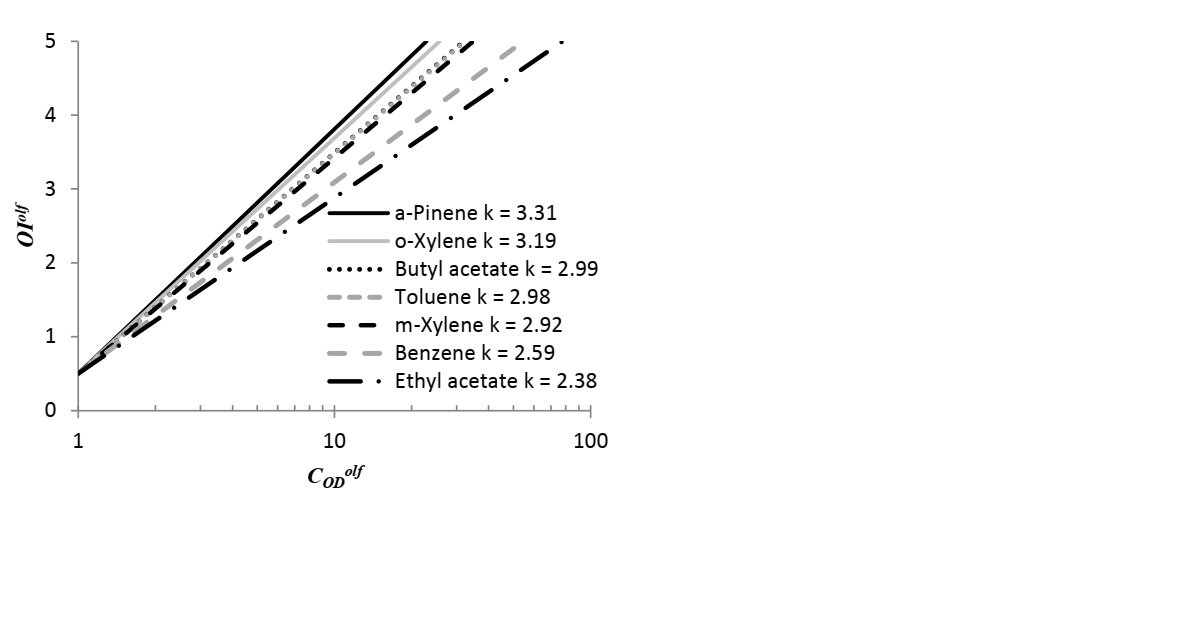
\includegraphics[width=0.8\textwidth]{Fig1.jpg}
    \caption{Descripción de la figura de ejemplo.}
    \label{fig:ejemplo}
\end{figure}

\subsection{Ejemplo de Tabla}
En la \refer{Tabla}{tab:ejemplo} se muestran los datos cargados desde un archivo CSV.

\begin{table}[H]
    \centering
    \caption{Datos de ejemplo cargados desde CSV.}
    \label{tab:ejemplo}
    \begin{adjustbox}{max width=\textwidth}
        \csvautotabular{tables/table.csv}
    \end{adjustbox}
\end{table}

CONTENIDO ADICIONAL DEL CAPÍTULO


\chapter{TITULO DEL CAPITULO}
\section{Introducción}
CONTENIDO SECCIÓN


\chapter{TITULO DEL CAPITULO}
\section{Introducción}
CONTENIDO SECCIÓN


\chapter{TITULO DEL CAPITULO}
\section{Introducción}
CONTENIDO SECCIÓN


\chapter{TITULO DEL CAPITULO}
\section{Introducción}
CONTENIDO SECCIÓN


\chapter{TITULO DEL CAPITULO}
\section{Introducción}
CONTENIDO SECCIÓN


\chapter{Conclusiones}
\section{Conclusiones}
CONTENIDO SECCIÓN



\backmatter
\bibliographystyle{apalike}
\phantomsection
\addcontentsline{toc}{chapter}{Referencias}
\bibliography{template.bib}

\appendix
\chapter{Anexos}
\section{Sección de Anexo}
CONTENIDO SECCIÓN


\end{document}
